\section{Actions utilisateur} 

Le joueur va devoir allier un grand nombre d'actions par tour. Pour cela il aura la possibilité de choisir parmi les commandes suivantes : \\ \\
- Sélectionner un vaisseau :  \textbf{SelectShipCommand}. \\
- Déplacer un vaisseau :  \textbf{MoveCommand}.\\
- Attaquer un vaisseau ennemi :  \textbf{AttackCommand}. \\
- Coloniser une planète à l'aide d'un vaisseau :  \textbf{ColonizeCommand}. \\
- Construire un bâtiment ou un vaisseau :  \textbf{BuildBuildingCommand} ou  \textbf{BuildShipCommand}. \\
- Terminer son tour : \textbf{FinishTurnCommand}. \\ \\
Pour effectuer les commandes concernant un vaisseau, le joueur devra préalablement sélectionner le vaisseau avec lequel il veut effectuer une action.

\section{Action automatique}

A chaque fin de tour, le jeu va venir appeler la fonction "CheckWinnerCommand" afin de déterminer si oui ou non la partie doit s'arrêter.

\section{Description logicielle}

L'ensemble des commandes contiennent un constructeur permettant de leur attribuer leur commandID. \\
De plus, elles possèdent toutes la méthode "serialize" permettant de mettre sous format Json l'ensemble des informations utiles concernant la commande.

\subsection{Command}

Cette classe permet de décrire l'ensemble des commandes. \\
Elle contient 2 attributs, l'un pour préciser lequel des joueurs effectue les commandes, l'autre pour préciser l'ID de la commande, c'est à dire la commande à effectuer. La méthode "execute" est elle définie par la méthode du même nom appartenant à la classe fille dont il est question.\\
L'ensemble des commandes héritent de cette classe.\\

\begin{figure}[!h]
\centering
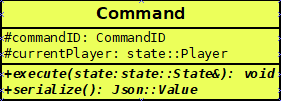
\includegraphics[width=0.5\textwidth]{pics/engine_pics/command.PNG}
\caption[Bloc "Command"]{\label{figure_simple}Bloc "Command"}
\end{figure}

\subsection{SelectShipCommand}

Cette commande permet de sélectionner le vaisseau "target" sur lequel on veut effectuer des actions.
La méthode execute vient vérifier si le vaisseau ciblé appartient bien au joueur effectuant la commande. Si c'est le cas elle permet alors l'affichage des différentes commandes permettant les actions du vaisseau.
\\
\begin{figure}[!h]
\centering
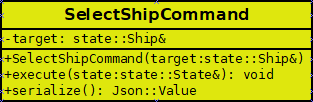
\includegraphics[width=0.5\textwidth]{pics/engine_pics/SelectShipCommand.PNG}
\caption[Bloc "SelectShipCommand"]{\label{figure_simple}Bloc "SelectShipCommand"}
\end{figure}

\subsection{MoveCommand}

Cette commande possède 2 attributs lui permettant de définir le vaisseau "ShipTarget" à déplacer et la position "PositionTarget" sur laquelle il souhaite le déplacer. \\
La méthode "execute" vient regarder si le déplacement est possible : \\
- aucun vaisseau allié est sur la position indiqué, \\
- la position ciblée est bien une SpaceCell de type "StellarSyst" ou "StellarWay", \\
- et enfin, si la position ciblée est bien dans la portée de déplacement du vaisseau. \\
Elle mets ensuite à jour la position du vaisseau ainsi que ses points de mouvement restants.
\\
\begin{figure}[!h]
\centering
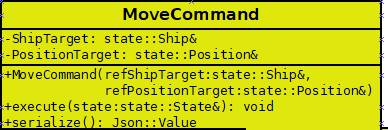
\includegraphics[width=0.5\textwidth]{pics/engine_pics/MoveCommand.PNG}
\caption[Bloc "MoveCommand"]{\label{figure_simple}Bloc "MoveCommand"}
\end{figure}

\subsection{AttackCommand}

Cette commande possède 2 attributs définissant le vaisseau "attacker" et le vaisseau "target". \\
La méthode "execute" vient vérifier que l'action d'attaque est bien possible c'est à dire que les 2 vaisseaux se trouvent bien sur la même position. Elle compare ensuite les types des vaisseaux pour actualiser l'état de chacun d'entre eux (destruction ou perte de point de vie).
\\
\begin{figure}[!h]
\centering
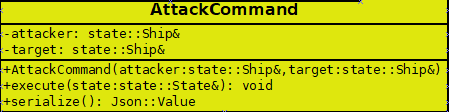
\includegraphics[width=0.5\textwidth]{pics/engine_pics/AttackCommand.PNG}
\caption[Bloc "AttackCommand"]{\label{figure_simple}Bloc "AttackCommand"}
\end{figure}

\subsection{BuildBuildingCommand et BuildShipCommand}

Ces 2 commandes ont un fonctionnement similaire. Elles permettent la construction d'un building ou d'un ship sur le système stellaire "StellarTarget". \\ La méthode "execute" vérifie si la construction est possible : \\
- StellarTarget est bien un système stellaire appartenant au joueur,\\
- et le joueur possède le nombre de ressources nécessaire à la construction. \\
La méthode ajoute donc l'objet construit à la liste de ship ou de building du joueur et actualise la production du système dans le cas de la construction du building.
\\
\begin{figure}[!h]
\centering
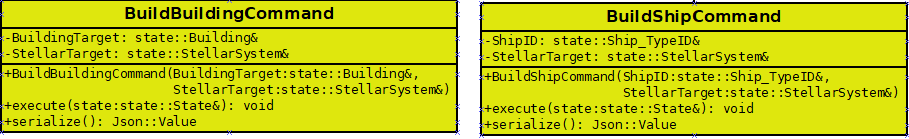
\includegraphics[width=1\textwidth]{pics/engine_pics/BuildsCommand.PNG}
\caption[Bloc "BuildBuildingCommand et BuildShipCommand"]{\label{figure_simple}Bloc "BuildBuildingCommand et BuildShipCommand"}
\end{figure}

\subsection{FinishTurnCommand}

Cette commande permet au joueur de mettre fin à son tour, d'incrémenter le nombre de tour dans la classe State pour permettre à l'autre joueur de jouer. \\
La méthode "execute" vérifie bien que c'est le joueur qui joue le tour qui effectue cette commande.

\begin{figure}[!h]
\centering
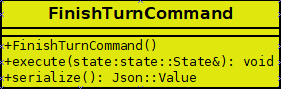
\includegraphics[width=0.5\textwidth]{pics/engine_pics/FinishTurnCommand.PNG}
\caption[Bloc "FinishTurnCommand"]{\label{figure_simple}Bloc "FinishTurnCommand"}
\end{figure}

\subsection{CheckWinnerCommand}

Cette commande permet à chaque fin de tour de vérifier si il y a un vainqueur. \\ 
La méthode "execute" vérifie que chacun des joueurs possèdent au moins 1 système stellaire ou 1 vaisseau. Dans le cas contraire il déclare vainqueur (victoire militaire) le joueur ayant toujours au moins un de ces objets. Si aucun joueur n'est gagnant à la fin d'un nombre de tour prédéfini (40 par exemple), alors il vient comparer les scores de chacun des joueurs pour déclarer gagnant le joueur ayant le plus de score.

\begin{figure}[!h]
\centering
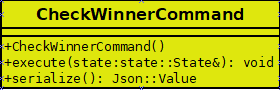
\includegraphics[width=0.5\textwidth]{pics/engine_pics/CheckWinnerCommand.PNG}
\caption[Bloc "CheckWinnerCommand"]{\label{figure_simple}Bloc "CheckWinnerCommand"}
\end{figure}